\documentclass[a4paper]{article}\usepackage[]{graphicx}\usepackage[]{color}
%% maxwidth is the original width if it is less than linewidth
%% otherwise use linewidth (to make sure the graphics do not exceed the margin)
\makeatletter
\def\maxwidth{ %
  \ifdim\Gin@nat@width>\linewidth
    \linewidth
  \else
    \Gin@nat@width
  \fi
}
\makeatother

\definecolor{fgcolor}{rgb}{0.345, 0.345, 0.345}
\newcommand{\hlnum}[1]{\textcolor[rgb]{0.686,0.059,0.569}{#1}}%
\newcommand{\hlstr}[1]{\textcolor[rgb]{0.192,0.494,0.8}{#1}}%
\newcommand{\hlcom}[1]{\textcolor[rgb]{0.678,0.584,0.686}{\textit{#1}}}%
\newcommand{\hlopt}[1]{\textcolor[rgb]{0,0,0}{#1}}%
\newcommand{\hlstd}[1]{\textcolor[rgb]{0.345,0.345,0.345}{#1}}%
\newcommand{\hlkwa}[1]{\textcolor[rgb]{0.161,0.373,0.58}{\textbf{#1}}}%
\newcommand{\hlkwb}[1]{\textcolor[rgb]{0.69,0.353,0.396}{#1}}%
\newcommand{\hlkwc}[1]{\textcolor[rgb]{0.333,0.667,0.333}{#1}}%
\newcommand{\hlkwd}[1]{\textcolor[rgb]{0.737,0.353,0.396}{\textbf{#1}}}%
\let\hlipl\hlkwb

\usepackage{framed}
\makeatletter
\newenvironment{kframe}{%
 \def\at@end@of@kframe{}%
 \ifinner\ifhmode%
  \def\at@end@of@kframe{\end{minipage}}%
  \begin{minipage}{\columnwidth}%
 \fi\fi%
 \def\FrameCommand##1{\hskip\@totalleftmargin \hskip-\fboxsep
 \colorbox{shadecolor}{##1}\hskip-\fboxsep
     % There is no \\@totalrightmargin, so:
     \hskip-\linewidth \hskip-\@totalleftmargin \hskip\columnwidth}%
 \MakeFramed {\advance\hsize-\width
   \@totalleftmargin\z@ \linewidth\hsize
   \@setminipage}}%
 {\par\unskip\endMakeFramed%
 \at@end@of@kframe}
\makeatother

\definecolor{shadecolor}{rgb}{.97, .97, .97}
\definecolor{messagecolor}{rgb}{0, 0, 0}
\definecolor{warningcolor}{rgb}{1, 0, 1}
\definecolor{errorcolor}{rgb}{1, 0, 0}
\newenvironment{knitrout}{}{} % an empty environment to be redefined in TeX

\usepackage{alltt}
\usepackage[margin=1in]{geometry}
\IfFileExists{upquote.sty}{\usepackage{upquote}}{}
\begin{document}
% ---- Beginn Analysis -----
  \begin{center}
\section*{Analysis of Pixel-Wise Correlations}
\end{center}
So far we've only looked at the mean stain levels between different patients. However, this ignores any spatial processes that might play a role. In order to start gaining a first insight into what spatial processes might play a role we'll here analyse the pixel-wise correlation matrices for the cores from different patients. This will for example highlight the presence/absence of specific cell types/meta-phenotypes.

% =======================================================
\section{A First Look at the Data}
I compute the correlation matrices using python and save the lower triangular parts of these matrices to file. In order to adjust for the different scales of the stains  I calculate the standardised correlations using the \texttt{np.corrcoef()} function.

Let's load in the results and label the columns with the correlation they measure:
\begin{knitrout}
\definecolor{shadecolor}{rgb}{0.969, 0.969, 0.969}\color{fgcolor}\begin{kframe}
\begin{alltt}
\hlstd{corrArr} \hlkwb{=} \hlkwd{read.csv}\hlstd{(}\hlstr{"pixelcorrelations.csv"}\hlstd{,}\hlkwc{header}\hlstd{=F)}
\hlkwd{dim}\hlstd{(corrArr)}
\end{alltt}
\begin{verbatim}
## [1] 121 668
\end{verbatim}
\begin{alltt}
\hlcom{# Label the columns}
\hlstd{labelArr} \hlkwb{=} \hlkwd{c}\hlstd{(}\hlstr{"CoreId"}\hlstd{,}\hlstr{"PtSnty"}\hlstd{)}
\hlstd{markerLabelsVec} \hlkwb{=} \hlkwd{c}\hlstd{(}\hlstr{'SrBCK'}\hlstd{,} \hlstr{'RR101'}\hlstd{,} \hlstr{'RR102'}\hlstd{,} \hlstr{'AvantiLipid'}\hlstd{,} \hlstr{'XeBCK'}\hlstd{,} \hlstr{'CD196'}\hlstd{,} \hlstr{'CD19'}\hlstd{,} \hlstr{'Vimentin'}\hlstd{,}
                    \hlstr{'CD163'}\hlstd{,} \hlstr{'CD20'}\hlstd{,} \hlstr{'CD16'}\hlstd{,} \hlstr{'CD25'}\hlstd{,} \hlstr{'p53'}\hlstd{,} \hlstr{'CD134'}\hlstd{,} \hlstr{'CD45'}\hlstd{,} \hlstr{'CD44s'}\hlstd{,} \hlstr{'CD14'}\hlstd{,} \hlstr{'FoxP3'}\hlstd{,}
                    \hlstr{'CD4'}\hlstd{,} \hlstr{'E-cadherin'}\hlstd{,} \hlstr{'p21'}\hlstd{,} \hlstr{'CD152'}\hlstd{,} \hlstr{'CD8a'}\hlstd{,} \hlstr{'CD11b'}\hlstd{,} \hlstr{'Beta-catenin'}\hlstd{,} \hlstr{'B7-H4'}\hlstd{,} \hlstr{'Ki67'}\hlstd{,}
                    \hlstr{'CollagenI'}\hlstd{,} \hlstr{'CD3'}\hlstd{,} \hlstr{'CD68'}\hlstd{,} \hlstr{'PD-L2'}\hlstd{,} \hlstr{'B7-H3'}\hlstd{,} \hlstr{'HLA-DR'}\hlstd{,} \hlstr{'pS6'}\hlstd{,} \hlstr{'HistoneH3'}\hlstd{,} \hlstr{'DNA191'}\hlstd{,}
                    \hlstr{'DNA193'}\hlstd{)}
\hlkwa{for} \hlstd{(i} \hlkwa{in} \hlkwd{seq}\hlstd{(}\hlnum{2}\hlstd{,}\hlnum{37}\hlstd{)) \{}
  \hlkwa{for} \hlstd{(j} \hlkwa{in} \hlkwd{seq}\hlstd{(i}\hlopt{-}\hlnum{1}\hlstd{)) \{}
    \hlstd{labelArr} \hlkwb{=} \hlkwd{c}\hlstd{(labelArr,}\hlkwd{paste0}\hlstd{(markerLabelsVec[i],}\hlstr{"."}\hlstd{,markerLabelsVec[j]))}
  \hlstd{\}}
\hlstd{\}}
\hlkwd{names}\hlstd{(corrArr)} \hlkwb{=} \hlstd{labelArr}
\end{alltt}
\end{kframe}
\end{knitrout}

Let's plot the correlations for each patient to see if there's an obvious difference between responders and non-responders.

\begin{knitrout}
\definecolor{shadecolor}{rgb}{0.969, 0.969, 0.969}\color{fgcolor}\begin{kframe}
\begin{alltt}
\hlkwd{library}\hlstd{(ggplot2)}
\hlkwd{library}\hlstd{(reshape2)}
\hlstd{corrArr} \hlkwb{=} \hlstd{corrArr[}\hlkwd{with}\hlstd{(corrArr,} \hlkwd{order}\hlstd{(PtSnty)), ]}
\hlstd{corrArr_idxd} \hlkwb{=} \hlkwd{data.frame}\hlstd{(corrArr,}\hlkwc{LinId}\hlstd{=}\hlkwd{seq}\hlstd{(}\hlkwd{nrow}\hlstd{(corrArr)))}
\hlstd{corrArr_reshaped} \hlkwb{=} \hlkwd{melt}\hlstd{(corrArr_idxd[,}\hlopt{-}\hlnum{1}\hlstd{],}\hlkwc{id.vars}\hlstd{=}\hlkwd{c}\hlstd{(}\hlstr{"LinId"}\hlstd{))}
\hlkwd{ggplot}\hlstd{(corrArr_reshaped,} \hlkwd{aes}\hlstd{(variable, LinId))} \hlopt{+}
  \hlkwd{geom_tile}\hlstd{(}\hlkwd{aes}\hlstd{(}\hlkwc{fill} \hlstd{= value),}\hlkwc{colour}\hlstd{=}\hlstr{"white"}\hlstd{)} \hlopt{+}
  \hlkwd{scale_fill_gradient}\hlstd{(}\hlkwc{low}\hlstd{=}\hlstr{"white"}\hlstd{,}\hlkwc{high}\hlstd{=}\hlstr{"steelblue"}\hlstd{)} \hlopt{+}
  \hlkwd{theme_bw}\hlstd{()} \hlopt{+}
  \hlkwd{labs}\hlstd{(}\hlkwc{x}\hlstd{=}\hlstr{""}\hlstd{,}\hlkwc{y}\hlstd{=}\hlstr{"Core"}\hlstd{)} \hlopt{+}
  \hlkwd{theme}\hlstd{(}\hlkwc{axis.text.x} \hlstd{=} \hlkwd{element_text}\hlstd{(}\hlkwc{angle}\hlstd{=}\hlnum{90}\hlstd{,} \hlkwc{hjust}\hlstd{=}\hlnum{1}\hlstd{))}
\end{alltt}
\end{kframe}\begin{figure}[h]
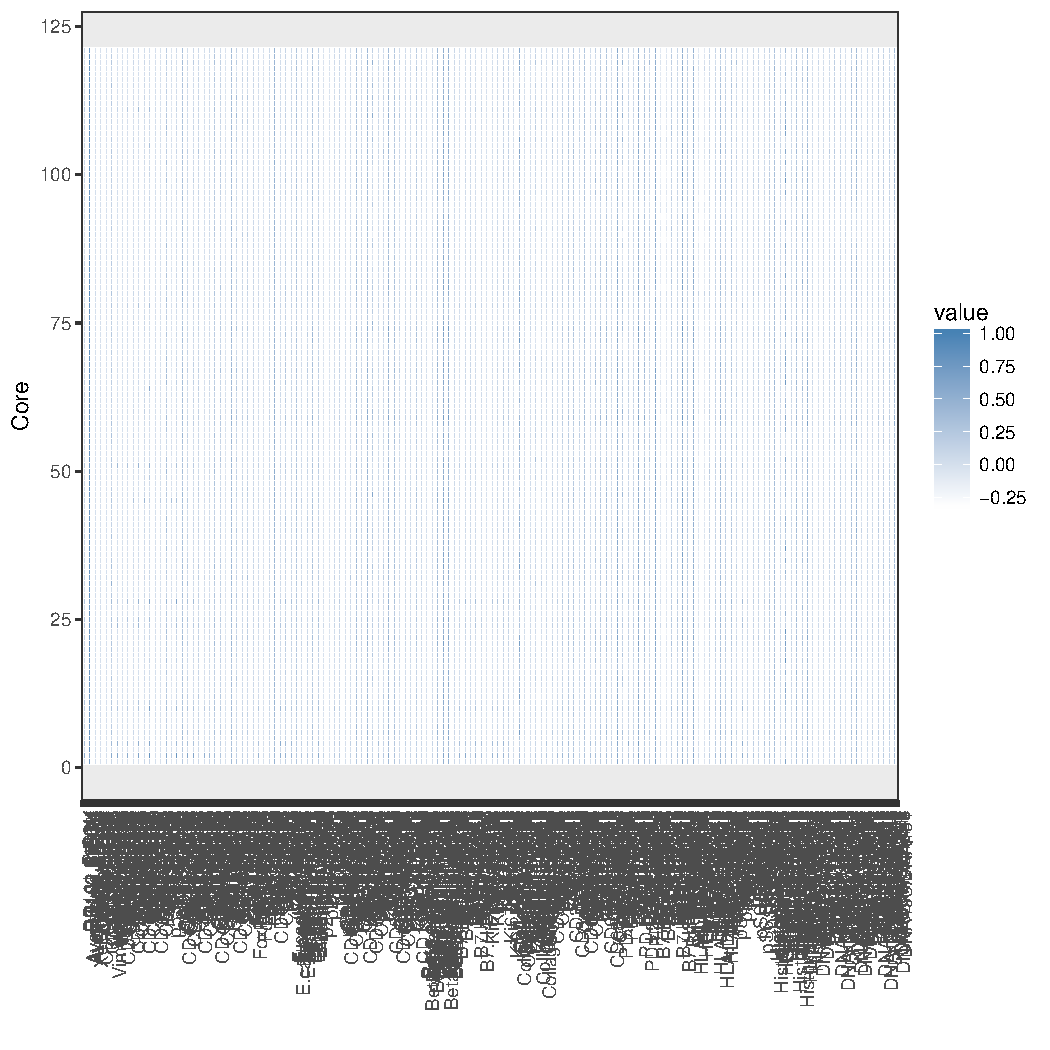
\includegraphics[width=\maxwidth]{figure/Fig_CorrMatrices-1} \caption[Pixel-wise correlation of the different stains for responders (top-half) and non-responders (bottom-half)]{Pixel-wise correlation of the different stains for responders (top-half) and non-responders (bottom-half).}\label{fig:Fig_CorrMatrices}
\end{figure}


\end{knitrout}

There doesn't seem anything obvious.
Let's test for statistically significant differences.


\section{A Logistic Regression Model}
Let's use a logistic regression model to find if there are any significant differences in the correlations between responders and non-responders.

\begin{knitrout}
\definecolor{shadecolor}{rgb}{0.969, 0.969, 0.969}\color{fgcolor}\begin{kframe}
\begin{alltt}
\hlstd{initModel} \hlkwb{=} \hlkwd{glm}\hlstd{(PtSnty} \hlopt{~}\hlstd{.,}\hlkwc{family}\hlstd{=}\hlkwd{binomial}\hlstd{(}\hlkwc{link}\hlstd{=}\hlstr{'logit'}\hlstd{),}
                \hlkwc{data}\hlstd{=corrArr)}
\end{alltt}


{\ttfamily\noindent\color{warningcolor}{\#\# Warning: glm.fit: algorithm did not converge}}\end{kframe}
\end{knitrout}

There seems to be a lot of co-linearity which prevents the model from being fitted. Maybe there are too many optima...

Let's try de-correlate the data. Since we can't compute VIFs, let's start by working with the correlation matrix. Remove any variables that are highly correlated with other variables. This stack-exchange post (https://stackoverflow.com/questions/18275639/remove-highly-correlated-variables) suggests a caret function. Let's try it:

\begin{knitrout}
\definecolor{shadecolor}{rgb}{0.969, 0.969, 0.969}\color{fgcolor}\begin{kframe}
\begin{alltt}
\hlkwd{library}\hlstd{(caret)}
\end{alltt}


{\ttfamily\noindent\itshape\color{messagecolor}{\#\# Loading required package: lattice}}\begin{alltt}
\hlstd{covariatesArr} \hlkwb{=} \hlstd{corrArr[,}\hlopt{-}\hlkwd{c}\hlstd{(}\hlnum{1}\hlstd{,}\hlnum{2}\hlstd{)]}
\hlstd{coMat} \hlkwb{=} \hlkwd{cor}\hlstd{(covariatesArr)}
\hlstd{hc} \hlkwb{=} \hlkwd{findCorrelation}\hlstd{(coMat,}\hlkwc{cutoff}\hlstd{=}\hlnum{0.7}\hlstd{,}\hlkwc{exact}\hlstd{=}\hlnum{TRUE}\hlstd{)} \hlcom{# put any value as a "cutoff" }
\hlstd{hc} \hlkwb{=} \hlkwd{sort}\hlstd{(hc)}
\hlstd{corrArr_Reduced} \hlkwb{=} \hlkwd{data.frame}\hlstd{(corrArr[,}\hlkwd{c}\hlstd{(}\hlnum{1}\hlstd{,}\hlnum{2}\hlstd{)],covariatesArr[,}\hlopt{-}\hlkwd{c}\hlstd{(hc)])}
\hlkwd{dim}\hlstd{(corrArr_Reduced)}
\end{alltt}
\begin{verbatim}
## [1] 121  76
\end{verbatim}
\end{kframe}
\end{knitrout}

Let's try fitting a model again.
\begin{knitrout}
\definecolor{shadecolor}{rgb}{0.969, 0.969, 0.969}\color{fgcolor}\begin{kframe}
\begin{alltt}
\hlstd{initModel} \hlkwb{=} \hlkwd{glm}\hlstd{(PtSnty} \hlopt{~}\hlstd{.,}\hlkwc{family}\hlstd{=}\hlkwd{binomial}\hlstd{(}\hlkwc{link}\hlstd{=}\hlstr{'logit'}\hlstd{),}
                \hlkwc{control} \hlstd{=} \hlkwd{list}\hlstd{(}\hlkwc{maxit} \hlstd{=} \hlnum{100}\hlstd{),}
                \hlkwc{data}\hlstd{=corrArr_Reduced)}
\end{alltt}


{\ttfamily\noindent\color{warningcolor}{\#\# Warning: glm.fit: fitted probabilities numerically 0 or 1 occurred}}\begin{alltt}
\hlkwd{summary}\hlstd{(initModel)}
\end{alltt}
\begin{verbatim}
## 
## Call:
## glm(formula = PtSnty ~ ., family = binomial(link = "logit"), 
##     data = corrArr_Reduced, control = list(maxit = 100))
## 
## Deviance Residuals: 
##        Min          1Q      Median          3Q         Max  
## -3.923e-06  -2.110e-08   2.110e-08   1.514e-06   4.288e-06  
## 
## Coefficients:
##                        Estimate Std. Error z value Pr(>|z|)
## (Intercept)           1.344e+02  8.903e+06       0        1
## CoreId               -3.416e-01  1.159e+04       0        1
## AvantiLipid.RR102     1.636e+02  5.743e+06       0        1
## CD196.SrBCK          -3.671e+02  1.088e+08       0        1
## CD196.XeBCK          -2.319e+03  6.183e+07       0        1
## CD19.CD196            7.670e+01  9.137e+06       0        1
## Vimentin.XeBCK       -7.413e+03  6.014e+08       0        1
## Vimentin.CD196       -3.712e+02  8.639e+06       0        1
## Vimentin.CD19        -2.440e+02  3.443e+07       0        1
## CD163.XeBCK           3.459e+03  4.876e+08       0        1
## CD16.CD196            2.096e+01  6.055e+07       0        1
## CD25.XeBCK            1.950e+03  2.244e+08       0        1
## CD25.CD196            3.676e+02  8.925e+06       0        1
## CD25.CD19            -1.749e+02  5.415e+06       0        1
## p53.CD196            -5.312e+02  3.677e+07       0        1
## p53.CD20             -6.319e+02  1.307e+07       0        1
## CD45.CD25            -9.419e+02  2.634e+08       0        1
## CD44s.AvantiLipid     2.065e+02  1.319e+07       0        1
## CD44s.CD196           5.248e+02  2.413e+07       0        1
## CD44s.Vimentin       -3.300e+02  1.771e+07       0        1
## CD44s.CD20            3.495e+02  2.386e+07       0        1
## CD44s.p53             4.463e+02  3.932e+07       0        1
## CD14.Vimentin         7.197e+02  1.166e+07       0        1
## CD14.CD16             1.275e+01  1.335e+07       0        1
## CD14.CD44s            1.604e+02  9.006e+06       0        1
## FoxP3.XeBCK           9.015e+02  1.399e+08       0        1
## FoxP3.CD19            1.018e+02  7.634e+06       0        1
## E.cadherin.CD196     -7.354e+02  9.047e+06       0        1
## E.cadherin.FoxP3      7.302e+02  7.729e+07       0        1
## CD152.AvantiLipid    -1.295e+02  2.067e+07       0        1
## CD152.CD163          -1.426e+03  6.374e+07       0        1
## CD152.E.cadherin     -2.238e+02  1.201e+07       0        1
## CD8a.CD196            4.430e+02  1.295e+07       0        1
## CD8a.CD25             7.373e+02  1.016e+07       0        1
## CD8a.CD14             6.357e+02  8.246e+06       0        1
## CD11b.CD44s          -6.163e+02  1.345e+07       0        1
## Beta.catenin.p53     -3.388e+02  1.155e+07       0        1
## B7.H4.E.cadherin     -4.870e+00  2.817e+07       0        1
## Ki67.AvantiLipid      4.265e+03  8.133e+07       0        1
## Ki67.p53              5.929e+02  4.184e+07       0        1
## CollagenI.SrBCK      -8.634e+02  5.406e+07       0        1
## CollagenI.XeBCK       2.907e+03  2.904e+08       0        1
## CollagenI.CD196       9.256e+01  3.603e+06       0        1
## CollagenI.CD19       -2.138e+02  4.469e+07       0        1
## CollagenI.CD163      -1.110e+03  1.238e+08       0        1
## CollagenI.p53         2.193e+02  4.543e+07       0        1
## CollagenI.CD45        1.791e+02  2.486e+07       0        1
## CollagenI.CD44s       1.585e+02  1.379e+07       0        1
## CollagenI.CD4        -3.040e+02  3.494e+07       0        1
## CD3.CD45             -3.213e+02  3.242e+07       0        1
## B7.H3.RR101          -5.465e+02  3.102e+07       0        1
## HLA.DR.SrBCK         -3.618e+02  4.750e+07       0        1
## HLA.DR.AvantiLipid   -1.413e+03  1.855e+07       0        1
## HLA.DR.Ki67          -4.861e+02  3.508e+07       0        1
## pS6.AvantiLipid      -7.810e+02  1.704e+07       0        1
## pS6.CD134             6.408e+01  5.361e+06       0        1
## pS6.HLA.DR            3.378e+02  2.262e+07       0        1
## HistoneH3.RR101       9.638e+01  6.528e+06       0        1
## HistoneH3.Vimentin   -2.272e+03  2.399e+07       0        1
## HistoneH3.CD20       -1.416e+03  3.515e+07       0        1
## HistoneH3.CD134       3.473e+02  1.294e+07       0        1
## HistoneH3.CD45       -7.034e+02  2.117e+07       0        1
## HistoneH3.CD44s       7.448e+02  1.840e+07       0        1
## HistoneH3.FoxP3       6.345e+02  9.344e+07       0        1
## HistoneH3.E.cadherin -1.408e+03  2.931e+07       0        1
## HistoneH3.p21         5.473e+02  2.818e+07       0        1
## HistoneH3.CollagenI   1.230e+03  2.195e+07       0        1
## DNA191.CD163          1.798e+03  9.048e+07       0        1
## DNA191.CD20           1.010e+03  6.875e+07       0        1
## DNA191.p53           -5.000e+02  4.245e+07       0        1
## DNA193.XeBCK          3.233e+03  3.018e+08       0        1
## DNA193.CD19          -7.426e+02  3.263e+07       0        1
## DNA193.FoxP3          1.075e+03  2.149e+07       0        1
## DNA193.Ki67          -2.017e+03  3.746e+07       0        1
## DNA193.HLA.DR         1.229e+03  1.961e+07       0        1
## DNA193.DNA191         8.968e+00  6.846e+06       0        1
## 
## (Dispersion parameter for binomial family taken to be 1)
## 
##     Null deviance: 1.6167e+02  on 120  degrees of freedom
## Residual deviance: 4.5840e-10  on  45  degrees of freedom
## AIC: 152
## 
## Number of Fisher Scoring iterations: 27
\end{verbatim}
\begin{alltt}
\hlcom{# Look at the VIFs}
\hlkwd{library}\hlstd{(car)}
\hlkwd{vif}\hlstd{(initModel)}
\end{alltt}
\begin{verbatim}
##               CoreId    AvantiLipid.RR102          CD196.SrBCK 
##            274.35914             68.25919           1954.29438 
##          CD196.XeBCK           CD19.CD196       Vimentin.XeBCK 
##            102.05953            274.98336           1557.08134 
##       Vimentin.CD196        Vimentin.CD19          CD163.XeBCK 
##            224.58496            357.88146           1218.78489 
##           CD16.CD196           CD25.XeBCK           CD25.CD196 
##           2312.59149            973.28338            761.41927 
##            CD25.CD19            p53.CD196             p53.CD20 
##            108.57328           3380.94038            255.96801 
##            CD45.CD25    CD44s.AvantiLipid          CD44s.CD196 
##           4649.79762            343.83970           1867.11544 
##       CD44s.Vimentin           CD44s.CD20            CD44s.p53 
##            765.94335            771.53682           1081.48400 
##        CD14.Vimentin            CD14.CD16           CD14.CD44s 
##            504.19056            147.77164            372.83141 
##          FoxP3.XeBCK           FoxP3.CD19     E.cadherin.CD196 
##             73.89555             80.58028            312.58433 
##     E.cadherin.FoxP3    CD152.AvantiLipid          CD152.CD163 
##           3448.22071           1210.87395           1377.49540 
##     CD152.E.cadherin           CD8a.CD196            CD8a.CD25 
##            772.99695           1433.62996             76.45263 
##            CD8a.CD14          CD11b.CD44s     Beta.catenin.p53 
##            520.64894            206.49233            343.10751 
##     B7.H4.E.cadherin     Ki67.AvantiLipid             Ki67.p53 
##            641.89802           3154.26256           5788.75184 
##      CollagenI.SrBCK      CollagenI.XeBCK      CollagenI.CD196 
##            236.73695           1529.22184            238.72848 
##       CollagenI.CD19      CollagenI.CD163        CollagenI.p53 
##           2790.62066           1658.11388           2179.86355 
##       CollagenI.CD45      CollagenI.CD44s        CollagenI.CD4 
##            182.18580            304.64228           2983.36298 
##             CD3.CD45          B7.H3.RR101         HLA.DR.SrBCK 
##           1983.57259           4779.22317           6153.76017 
##   HLA.DR.AvantiLipid          HLA.DR.Ki67      pS6.AvantiLipid 
##           1039.58441           2740.51106            349.97523 
##            pS6.CD134           pS6.HLA.DR      HistoneH3.RR101 
##            135.44281           1209.71779            142.41971 
##   HistoneH3.Vimentin       HistoneH3.CD20      HistoneH3.CD134 
##            699.20282            622.34000            333.71593 
##       HistoneH3.CD45      HistoneH3.CD44s      HistoneH3.FoxP3 
##            260.51664            513.92370           4363.62660 
## HistoneH3.E.cadherin        HistoneH3.p21  HistoneH3.CollagenI 
##           2812.36908            905.03840           1040.90722 
##         DNA191.CD163          DNA191.CD20           DNA191.p53 
##           1119.80585            690.10707           5483.24577 
##         DNA193.XeBCK          DNA193.CD19         DNA193.FoxP3 
##            591.36331            621.73769            186.65420 
##          DNA193.Ki67        DNA193.HLA.DR        DNA193.DNA191 
##           1370.72245           2329.65186            727.66523
\end{verbatim}
\end{kframe}
\end{knitrout}

Pretty high VIFs, but let's do a stepping search.

\begin{knitrout}
\definecolor{shadecolor}{rgb}{0.969, 0.969, 0.969}\color{fgcolor}\begin{kframe}
\begin{alltt}
\hlkwd{source}\hlstd{(}\hlstr{"../Utils_Maxi.R"}\hlstd{)}
\hlstd{reducedCoLinModelArr200} \hlkwb{=} \hlkwd{AICVIFCoElimination}\hlstd{(}\hlkwd{DecorrelateVariables}\hlstd{(initModel,}\hlnum{200}\hlstd{,}\hlkwc{verbose}\hlstd{=F)}
                                              \hlstd{,}\hlkwc{verbose}\hlstd{=F)}
\hlstd{reducedCoLinModelArr100} \hlkwb{=} \hlkwd{AICVIFCoElimination}\hlstd{(}\hlkwd{DecorrelateVariables}\hlstd{(initModel,}\hlnum{100}\hlstd{,}\hlkwc{verbose}\hlstd{=F)}
                                              \hlstd{,}\hlkwc{verbose}\hlstd{=F)}
\hlstd{reducedCoLinModelArr20} \hlkwb{=} \hlkwd{AICVIFCoElimination}\hlstd{(}\hlkwd{DecorrelateVariables}\hlstd{(initModel,}\hlnum{20}\hlstd{,}\hlkwc{verbose}\hlstd{=F)}
                                             \hlstd{,}\hlkwc{verbose}\hlstd{=F)}
\hlstd{reducedCoLinModelArr10} \hlkwb{=} \hlkwd{AICVIFCoElimination}\hlstd{(}\hlkwd{DecorrelateVariables}\hlstd{(initModel,}\hlnum{10}\hlstd{,}\hlkwc{verbose}\hlstd{=F)}
                                             \hlstd{,}\hlkwc{verbose}\hlstd{=F)}
\end{alltt}
\end{kframe}
\end{knitrout}

Say we tolerate a maximum VIF of 25. What are the best AICs we get?

\begin{knitrout}
\definecolor{shadecolor}{rgb}{0.969, 0.969, 0.969}\color{fgcolor}\begin{kframe}
\begin{alltt}
\hlstd{targetVIF} \hlkwb{=} \hlnum{25}
\hlstd{best200} \hlkwb{=} \hlstd{reducedCoLinModelArr200[}\hlkwd{unlist}\hlstd{(reducedCoLinModelArr200}\hlopt{$}\hlstd{maxVIF)}\hlopt{<}\hlstd{targetVIF,]}
\hlstd{best200} \hlkwb{=} \hlstd{best200[}\hlkwd{which.min}\hlstd{(}\hlkwd{unlist}\hlstd{(best200}\hlopt{$}\hlstd{V1)),]}
\hlstd{best100} \hlkwb{=} \hlstd{reducedCoLinModelArr100[}\hlkwd{unlist}\hlstd{(reducedCoLinModelArr100}\hlopt{$}\hlstd{maxVIF)}\hlopt{<}\hlstd{targetVIF,]}
\hlstd{best100} \hlkwb{=} \hlstd{best100[}\hlkwd{which.min}\hlstd{(}\hlkwd{unlist}\hlstd{(best100}\hlopt{$}\hlstd{V1)),]}
\hlstd{best20} \hlkwb{=} \hlstd{reducedCoLinModelArr20[}\hlkwd{unlist}\hlstd{(reducedCoLinModelArr20}\hlopt{$}\hlstd{maxVIF)}\hlopt{<}\hlstd{targetVIF,]}
\hlstd{best20} \hlkwb{=} \hlstd{best20[}\hlkwd{which.min}\hlstd{(}\hlkwd{unlist}\hlstd{(best20}\hlopt{$}\hlstd{V1)),]}
\hlstd{best10} \hlkwb{=} \hlstd{reducedCoLinModelArr10[}\hlkwd{unlist}\hlstd{(reducedCoLinModelArr10}\hlopt{$}\hlstd{maxVIF)}\hlopt{<}\hlstd{targetVIF,]}
\hlstd{best10} \hlkwb{=} \hlstd{best10[}\hlkwd{which.min}\hlstd{(}\hlkwd{unlist}\hlstd{(best10}\hlopt{$}\hlstd{V1)),]}
\hlkwd{print}\hlstd{(best200[}\hlnum{1}\hlopt{:}\hlnum{4}\hlstd{])}
\end{alltt}
\begin{verbatim}
##         V1  accuracy   maxVIF nVariables
## 5 139.1947 0.7933884 4.558939         14
\end{verbatim}
\begin{alltt}
\hlkwd{print}\hlstd{(best100[}\hlnum{1}\hlopt{:}\hlnum{4}\hlstd{])}
\end{alltt}
\begin{verbatim}
##         V1  accuracy   maxVIF nVariables
## 5 139.1947 0.7933884 4.558939         14
\end{verbatim}
\begin{alltt}
\hlkwd{print}\hlstd{(best20[}\hlnum{1}\hlopt{:}\hlnum{4}\hlstd{])}
\end{alltt}
\begin{verbatim}
##         V1  accuracy   maxVIF nVariables
## 1 147.5249 0.7024793 16.69107          8
\end{verbatim}
\begin{alltt}
\hlkwd{print}\hlstd{(best10[}\hlnum{1}\hlopt{:}\hlnum{4}\hlstd{])}
\end{alltt}
\begin{verbatim}
##         V1  accuracy   maxVIF nVariables
## 1 144.6403 0.7107438 8.840991          8
\end{verbatim}
\end{kframe}
\end{knitrout}

Nice, so we get a model with fairly de-correlated variables (maxVIF around xxx) and pretty decent predictive power (around xxx) accuracy)!

What does the model consist of?

\begin{knitrout}
\definecolor{shadecolor}{rgb}{0.969, 0.969, 0.969}\color{fgcolor}\begin{kframe}
\begin{alltt}
\hlstd{best100Model} \hlkwb{=} \hlkwd{glm}\hlstd{(}\hlkwd{paste0}\hlstd{(best100[,}\hlnum{5}\hlstd{]),}\hlkwc{family}\hlstd{=}\hlkwd{binomial}\hlstd{(}\hlkwc{link}\hlstd{=}\hlstr{'logit'}\hlstd{),}
                           \hlkwc{data}\hlstd{=corrArr_Reduced)}
\hlkwd{PlotCoefficients}\hlstd{(best10Model,}\hlkwc{yLim}\hlstd{=}\hlkwd{c}\hlstd{(}\hlopt{-}\hlnum{30}\hlstd{,}\hlnum{30}\hlstd{),}\hlkwc{yPos}\hlstd{=}\hlnum{22}\hlstd{,}\hlkwc{errBarWidth}\hlstd{=}\hlnum{.4}\hlstd{)}
\end{alltt}


{\ttfamily\noindent\bfseries\color{errorcolor}{\#\# Error in PlotCoefficients(best10Model, yLim = c(-30, 30), yPos = 22, errBarWidth = 0.4): object 'best10Model' not found}}\end{kframe}
\end{knitrout}

Strange... It's picking up XeBCK which should be background control. 

% =======================================================
\section{Cleaning up the Data}
I just spoke to Olya and I now know all the different stains. They are all meaningful to a certain extend, but there is a certain amount of redundancy in them. Let's clean the data up to remove some of that redundancy.
\begin{knitrout}
\definecolor{shadecolor}{rgb}{0.969, 0.969, 0.969}\color{fgcolor}\begin{kframe}
\begin{alltt}
\hlstd{stainsToOmitVec} \hlkwb{=} \hlkwd{c}\hlstd{(}\hlstr{'SrBCK'}\hlstd{,}\hlstr{'RR101'}\hlstd{,}\hlstr{'XeBCK'}\hlstd{,}\hlstr{'DNA193'}\hlstd{)}
\hlstd{colToOmitVec} \hlkwb{=} \hlkwd{c}\hlstd{()}

\hlcom{# Calculate the index of the columns with correlations with the above stains and }
\hlcom{# collect them in a vector.}
\hlstd{k} \hlkwb{=} \hlnum{3}
\hlkwa{for} \hlstd{(i} \hlkwa{in} \hlkwd{seq}\hlstd{(}\hlnum{2}\hlstd{,}\hlnum{37}\hlstd{)) \{}
  \hlkwa{for} \hlstd{(j} \hlkwa{in} \hlkwd{seq}\hlstd{(i}\hlopt{-}\hlnum{1}\hlstd{)) \{}
    \hlkwa{if} \hlstd{(}\hlkwd{any}\hlstd{(markerLabelsVec[}\hlkwd{c}\hlstd{(i,j)]} \hlopt \hlstd{stainsToOmitVec)) \{}
      \hlstd{colToOmitVec} \hlkwb{=} \hlkwd{c}\hlstd{(colToOmitVec,k)}
    \hlstd{\}}
    \hlstd{k} \hlkwb{=} \hlstd{k} \hlopt{+} \hlnum{1}
  \hlstd{\}}
\hlstd{\}}

\hlstd{corrArr_Curated} \hlkwb{=} \hlstd{corrArr[,}\hlopt{-}\hlstd{colToOmitVec]}
\hlkwd{dim}\hlstd{(corrArr_Curated)} \hlcom{# Should be removing 36*4-4*3/2 = 138, so expect 530}
\end{alltt}
\begin{verbatim}
## [1] 121 530
\end{verbatim}
\end{kframe}
\end{knitrout}

Let's do de-correlation:
\begin{knitrout}
\definecolor{shadecolor}{rgb}{0.969, 0.969, 0.969}\color{fgcolor}\begin{kframe}
\begin{alltt}
\hlstd{covariatesArr} \hlkwb{=} \hlstd{corrArr_Curated[,}\hlopt{-}\hlkwd{c}\hlstd{(}\hlnum{1}\hlstd{,}\hlnum{2}\hlstd{)]}
\hlstd{coMat} \hlkwb{=} \hlkwd{cor}\hlstd{(covariatesArr)}
\hlstd{hc} \hlkwb{=} \hlkwd{findCorrelation}\hlstd{(coMat,}\hlkwc{cutoff}\hlstd{=}\hlnum{0.7}\hlstd{,}\hlkwc{exact}\hlstd{=}\hlnum{TRUE}\hlstd{)} \hlcom{# put any value as a "cutoff" }
\hlstd{hc} \hlkwb{=} \hlkwd{sort}\hlstd{(hc)}
\hlstd{corrArrCurated_Reduced} \hlkwb{=} \hlkwd{data.frame}\hlstd{(corrArr_Curated[,}\hlkwd{c}\hlstd{(}\hlnum{1}\hlstd{,}\hlnum{2}\hlstd{)],covariatesArr[,}\hlopt{-}\hlkwd{c}\hlstd{(hc)])}
\hlkwd{dim}\hlstd{(corrArrCurated_Reduced)}
\end{alltt}
\begin{verbatim}
## [1] 121  67
\end{verbatim}
\end{kframe}
\end{knitrout}

Let's try fitting a model again.
\begin{knitrout}
\definecolor{shadecolor}{rgb}{0.969, 0.969, 0.969}\color{fgcolor}\begin{kframe}
\begin{alltt}
\hlstd{initModel} \hlkwb{=} \hlkwd{glm}\hlstd{(PtSnty} \hlopt{~}\hlstd{.,}\hlkwc{family}\hlstd{=}\hlkwd{binomial}\hlstd{(}\hlkwc{link}\hlstd{=}\hlstr{'logit'}\hlstd{),}
                \hlkwc{control} \hlstd{=} \hlkwd{list}\hlstd{(}\hlkwc{maxit} \hlstd{=} \hlnum{100}\hlstd{),}
                \hlkwc{data}\hlstd{=corrArrCurated_Reduced[,}\hlopt{-}\hlnum{1}\hlstd{])}
\end{alltt}


{\ttfamily\noindent\color{warningcolor}{\#\# Warning: glm.fit: fitted probabilities numerically 0 or 1 occurred}}\begin{alltt}
\hlkwd{summary}\hlstd{(initModel)}
\end{alltt}
\begin{verbatim}
## 
## Call:
## glm(formula = PtSnty ~ ., family = binomial(link = "logit"), 
##     data = corrArrCurated_Reduced[, -1], control = list(maxit = 100))
## 
## Deviance Residuals: 
##        Min          1Q      Median          3Q         Max  
## -5.552e-06  -2.110e-08   2.110e-08   1.121e-06   5.050e-06  
## 
## Coefficients:
##                          Estimate Std. Error z value Pr(>|z|)
## (Intercept)             3.405e+02  1.280e+07       0        1
## AvantiLipid.RR102       1.317e+00  7.363e+06       0        1
## CD19.CD196             -5.601e+02  7.556e+06       0        1
## Vimentin.CD196         -6.878e+02  1.351e+07       0        1
## Vimentin.CD19           2.909e+03  4.602e+07       0        1
## CD16.AvantiLipid       -1.798e+03  3.170e+07       0        1
## CD16.CD196              4.008e+01  5.607e+07       0        1
## CD25.CD196              8.684e+02  4.995e+06       0        1
## CD25.CD19               3.439e+02  5.642e+06       0        1
## CD25.CD163             -9.170e+03  7.482e+07       0        1
## p53.AvantiLipid         4.200e+00  1.479e+07       0        1
## p53.CD196              -1.038e+03  1.362e+07       0        1
## CD44s.AvantiLipid       4.999e+02  2.563e+07       0        1
## CD44s.CD196             7.765e+02  2.066e+07       0        1
## CD44s.Vimentin          2.546e-01  7.909e+06       0        1
## CD44s.CD16              4.344e+02  1.885e+07       0        1
## CD44s.p53               6.577e+02  1.713e+07       0        1
## CD14.Vimentin           9.333e+02  7.928e+06       0        1
## CD14.CD16               5.656e+01  5.480e+07       0        1
## CD14.CD134             -9.134e+01  8.754e+06       0        1
## CD14.CD44s              3.673e+02  1.224e+07       0        1
## FoxP3.CD19             -6.080e+01  5.718e+06       0        1
## CD4.p53                -3.973e+02  7.407e+06       0        1
## CD4.CD44s              -1.501e+03  1.833e+07       0        1
## E.cadherin.CD196       -4.787e+02  8.307e+06       0        1
## E.cadherin.FoxP3        1.985e+02  4.652e+07       0        1
## CD152.CD163            -9.288e+02  1.887e+07       0        1
## CD8a.AvantiLipid       -6.787e+01  1.852e+07       0        1
## CD8a.CD196              4.868e+02  5.200e+06       0        1
## CD8a.CD25              -1.092e+02  2.531e+07       0        1
## CD8a.E.cadherin         2.650e+02  9.350e+06       0        1
## CD11b.CD45             -1.829e+03  3.490e+07       0        1
## B7.H4.AvantiLipid       6.632e+02  7.476e+07       0        1
## Ki67.AvantiLipid        1.397e+03  5.332e+07       0        1
## Ki67.B7.H4             -1.278e+03  2.240e+07       0        1
## CollagenI.CD196         7.406e+01  4.564e+06       0        1
## CollagenI.CD19         -5.153e+02  1.112e+07       0        1
## CollagenI.CD163         1.095e+03  6.770e+07       0        1
## CollagenI.p53           2.492e+01  1.167e+07       0        1
## CollagenI.CD45          5.466e+02  2.579e+07       0        1
## CollagenI.CD44s        -2.569e+02  1.011e+07       0        1
## CollagenI.CD14         -2.147e+02  7.525e+06       0        1
## CollagenI.Beta.catenin -2.092e+02  8.784e+06       0        1
## B7.H3.RR102            -3.406e+02  1.097e+07       0        1
## HLA.DR.RR102            6.536e+02  3.298e+07       0        1
## HLA.DR.p53              1.996e+01  8.928e+06       0        1
## HLA.DR.Ki67             6.116e+02  1.979e+07       0        1
## pS6.AvantiLipid        -8.196e+02  2.210e+07       0        1
## pS6.CD134              -1.851e+02  5.026e+06       0        1
## pS6.HLA.DR              3.293e+02  1.690e+07       0        1
## HistoneH3.RR102        -3.525e+01  1.611e+07       0        1
## HistoneH3.Vimentin     -6.300e+02  3.165e+07       0        1
## HistoneH3.CD20         -1.863e+03  7.297e+07       0        1
## HistoneH3.CD134         2.839e+02  1.339e+07       0        1
## HistoneH3.CD45         -1.138e+03  3.145e+07       0        1
## HistoneH3.CD44s         1.112e+03  1.498e+07       0        1
## HistoneH3.p21           1.418e+03  1.795e+07       0        1
## HistoneH3.CD152        -1.130e+03  1.639e+07       0        1
## HistoneH3.B7.H4        -2.397e+02  3.157e+07       0        1
## HistoneH3.CollagenI     6.994e+02  1.542e+07       0        1
## HistoneH3.HLA.DR       -5.854e+02  1.693e+07       0        1
## DNA191.CD19             1.109e+03  3.681e+07       0        1
## DNA191.CD163           -5.344e+00  3.153e+07       0        1
## DNA191.CD20             3.272e+03  9.246e+07       0        1
## DNA191.FoxP3           -4.923e+02  1.854e+07       0        1
## DNA191.HLA.DR           5.183e+02  1.285e+07       0        1
## 
## (Dispersion parameter for binomial family taken to be 1)
## 
##     Null deviance: 1.6167e+02  on 120  degrees of freedom
## Residual deviance: 4.2703e-10  on  55  degrees of freedom
## AIC: 132
## 
## Number of Fisher Scoring iterations: 28
\end{verbatim}
\begin{alltt}
\hlcom{# Look at the VIFs}
\hlkwd{vif}\hlstd{(initModel)}
\end{alltt}
\begin{verbatim}
##      AvantiLipid.RR102             CD19.CD196         Vimentin.CD196 
##              100.15973              219.70611              495.54802 
##          Vimentin.CD19       CD16.AvantiLipid             CD16.CD196 
##              631.56673              279.07232             1609.11311 
##             CD25.CD196              CD25.CD19             CD25.CD163 
##              231.22305              165.44975              136.73243 
##        p53.AvantiLipid              p53.CD196      CD44s.AvantiLipid 
##              382.66081              481.22662              959.80087 
##            CD44s.CD196         CD44s.Vimentin             CD44s.CD16 
##             1146.46674              167.05345              223.04109 
##              CD44s.p53          CD14.Vimentin              CD14.CD16 
##              134.74573              174.23425             1805.15391 
##             CD14.CD134             CD14.CD44s             FoxP3.CD19 
##              364.87324              961.56553               21.00971 
##                CD4.p53              CD4.CD44s       E.cadherin.CD196 
##              167.42148              706.93091              402.95821 
##       E.cadherin.FoxP3            CD152.CD163       CD8a.AvantiLipid 
##              622.05083              122.53286              702.37535 
##             CD8a.CD196              CD8a.CD25        CD8a.E.cadherin 
##              350.03564              632.53709              414.57072 
##             CD11b.CD45      B7.H4.AvantiLipid       Ki67.AvantiLipid 
##              437.91610              623.99836             1355.56080 
##             Ki67.B7.H4        CollagenI.CD196         CollagenI.CD19 
##              467.23494              327.03865              158.66681 
##        CollagenI.CD163          CollagenI.p53         CollagenI.CD45 
##              389.17491              134.05468              115.64912 
##        CollagenI.CD44s         CollagenI.CD14 CollagenI.Beta.catenin 
##              141.13691              123.27490              276.12938 
##            B7.H3.RR102           HLA.DR.RR102             HLA.DR.p53 
##              358.40130             3930.97560             1025.99257 
##            HLA.DR.Ki67        pS6.AvantiLipid              pS6.CD134 
##             1210.47989              343.48040               96.12266 
##             pS6.HLA.DR        HistoneH3.RR102     HistoneH3.Vimentin 
##              419.03356              590.11377              618.96788 
##         HistoneH3.CD20        HistoneH3.CD134         HistoneH3.CD45 
##             1677.44839              260.58545              668.89301 
##        HistoneH3.CD44s          HistoneH3.p21        HistoneH3.CD152 
##              202.32437              247.04700              618.23921 
##        HistoneH3.B7.H4    HistoneH3.CollagenI       HistoneH3.HLA.DR 
##              362.90191              425.16517             2776.28349 
##            DNA191.CD19           DNA191.CD163            DNA191.CD20 
##              464.45397              114.82713              747.01580 
##           DNA191.FoxP3          DNA191.HLA.DR 
##              164.06612              448.21844
\end{verbatim}
\end{kframe}
\end{knitrout}

Pretty high VIFs, but let's do a stepping search.

\begin{knitrout}
\definecolor{shadecolor}{rgb}{0.969, 0.969, 0.969}\color{fgcolor}\begin{kframe}
\begin{alltt}
\hlstd{reducedCoLinModelArr200} \hlkwb{=} \hlkwd{AICVIFCoElimination}\hlstd{(}\hlkwd{DecorrelateVariables}\hlstd{(initModel,}\hlnum{200}\hlstd{,}\hlkwc{verbose}\hlstd{=F)}
                                              \hlstd{,}\hlkwc{verbose}\hlstd{=F)}
\hlstd{reducedCoLinModelArr100} \hlkwb{=} \hlkwd{AICVIFCoElimination}\hlstd{(}\hlkwd{DecorrelateVariables}\hlstd{(initModel,}\hlnum{100}\hlstd{,}\hlkwc{verbose}\hlstd{=F)}
                                              \hlstd{,}\hlkwc{verbose}\hlstd{=F)}
\hlstd{reducedCoLinModelArr20} \hlkwb{=} \hlkwd{AICVIFCoElimination}\hlstd{(}\hlkwd{DecorrelateVariables}\hlstd{(initModel,}\hlnum{20}\hlstd{,}\hlkwc{verbose}\hlstd{=F)}
                                             \hlstd{,}\hlkwc{verbose}\hlstd{=F)}
\hlstd{reducedCoLinModelArr10} \hlkwb{=} \hlkwd{AICVIFCoElimination}\hlstd{(}\hlkwd{DecorrelateVariables}\hlstd{(initModel,}\hlnum{10}\hlstd{,}\hlkwc{verbose}\hlstd{=F)}
                                             \hlstd{,}\hlkwc{verbose}\hlstd{=F)}
\hlcom{# Print out the results}
\hlstd{reducedCoLinModelArr200[,}\hlnum{1}\hlopt{:}\hlnum{4}\hlstd{]}
\end{alltt}
\begin{verbatim}
##         V1  accuracy   maxVIF nVariables
## 1 141.4547  0.768595 16.05183         15
## 2 151.3508 0.7438017 4.519692         14
## 3 150.3381 0.7190083 4.519692         13
## 4 160.2219 0.6942149 3.224513         12
## 5 151.9751 0.7190083 3.224513          6
## 6 156.1263 0.6694215  1.91365          5
## 7 153.0455  0.661157  1.91365          2
## 8 159.8677 0.6033058 1.003952          1
## 9 159.8677 0.6033058 1.003952          1
\end{verbatim}
\begin{alltt}
\hlstd{reducedCoLinModelArr100[,}\hlnum{1}\hlopt{:}\hlnum{4}\hlstd{]}
\end{alltt}
\begin{verbatim}
##         V1  accuracy   maxVIF nVariables
## 1 141.4547  0.768595 16.05183         15
## 2 151.3508 0.7438017 4.519692         14
## 3 150.3381 0.7190083 4.519692         13
## 4 160.2219 0.6942149 3.224513         12
## 5 151.9751 0.7190083 3.224513          6
## 6 156.1263 0.6694215  1.91365          5
## 7 153.0455  0.661157  1.91365          2
## 8 159.8677 0.6033058 1.003952          1
## 9 159.8677 0.6033058 1.003952          1
\end{verbatim}
\begin{alltt}
\hlstd{reducedCoLinModelArr20[,}\hlnum{1}\hlopt{:}\hlnum{4}\hlstd{]}
\end{alltt}
\begin{verbatim}
##         V1  accuracy   maxVIF nVariables
## 1 141.4547  0.768595 16.05183         15
## 2 151.3508 0.7438017 4.519692         14
## 3 150.3381 0.7190083 4.519692         13
## 4 160.2219 0.6942149 3.224513         12
## 5 151.9751 0.7190083 3.224513          6
## 6 156.1263 0.6694215  1.91365          5
## 7 153.0455  0.661157  1.91365          2
## 8 159.8677 0.6033058 1.003952          1
## 9 159.8677 0.6033058 1.003952          1
\end{verbatim}
\begin{alltt}
\hlstd{reducedCoLinModelArr10[,}\hlnum{1}\hlopt{:}\hlnum{4}\hlstd{]}
\end{alltt}
\begin{verbatim}
##         V1  accuracy   maxVIF nVariables
## 1 144.4886 0.7768595 9.742738         10
## 2 156.4682 0.7272727 2.460953          9
## 3 151.1057 0.7272727 2.460953          4
## 4 159.8545 0.6446281  2.22998          3
## 5 156.0279 0.6528926  2.22998          1
\end{verbatim}
\end{kframe}
\end{knitrout}

Say we tolerate a maximum VIF of 25. What are the best AICs we get?

\begin{knitrout}
\definecolor{shadecolor}{rgb}{0.969, 0.969, 0.969}\color{fgcolor}\begin{kframe}
\begin{alltt}
\hlstd{targetVIF} \hlkwb{=} \hlnum{5}
\hlstd{best200} \hlkwb{=} \hlstd{reducedCoLinModelArr200[}\hlkwd{unlist}\hlstd{(reducedCoLinModelArr200}\hlopt{$}\hlstd{maxVIF)}\hlopt{<}\hlstd{targetVIF,]}
\hlstd{best200} \hlkwb{=} \hlstd{best200[}\hlkwd{which.min}\hlstd{(}\hlkwd{unlist}\hlstd{(best200}\hlopt{$}\hlstd{V1)),]}
\hlstd{best100} \hlkwb{=} \hlstd{reducedCoLinModelArr100[}\hlkwd{unlist}\hlstd{(reducedCoLinModelArr100}\hlopt{$}\hlstd{maxVIF)}\hlopt{<}\hlstd{targetVIF,]}
\hlstd{best100} \hlkwb{=} \hlstd{best100[}\hlkwd{which.min}\hlstd{(}\hlkwd{unlist}\hlstd{(best100}\hlopt{$}\hlstd{V1)),]}
\hlstd{best20} \hlkwb{=} \hlstd{reducedCoLinModelArr20[}\hlkwd{unlist}\hlstd{(reducedCoLinModelArr20}\hlopt{$}\hlstd{maxVIF)}\hlopt{<}\hlstd{targetVIF,]}
\hlstd{best20} \hlkwb{=} \hlstd{best20[}\hlkwd{which.min}\hlstd{(}\hlkwd{unlist}\hlstd{(best20}\hlopt{$}\hlstd{V1)),]}
\hlstd{best10} \hlkwb{=} \hlstd{reducedCoLinModelArr10[}\hlkwd{unlist}\hlstd{(reducedCoLinModelArr10}\hlopt{$}\hlstd{maxVIF)}\hlopt{<}\hlstd{targetVIF,]}
\hlstd{best10} \hlkwb{=} \hlstd{best10[}\hlkwd{which.min}\hlstd{(}\hlkwd{unlist}\hlstd{(best10}\hlopt{$}\hlstd{V1)),]}
\hlkwd{print}\hlstd{(best200[}\hlnum{1}\hlopt{:}\hlnum{4}\hlstd{])}
\end{alltt}
\begin{verbatim}
##         V1  accuracy   maxVIF nVariables
## 3 150.3381 0.7190083 4.519692         13
\end{verbatim}
\begin{alltt}
\hlkwd{print}\hlstd{(best100[}\hlnum{1}\hlopt{:}\hlnum{4}\hlstd{])}
\end{alltt}
\begin{verbatim}
##         V1  accuracy   maxVIF nVariables
## 3 150.3381 0.7190083 4.519692         13
\end{verbatim}
\begin{alltt}
\hlkwd{print}\hlstd{(best20[}\hlnum{1}\hlopt{:}\hlnum{4}\hlstd{])}
\end{alltt}
\begin{verbatim}
##         V1  accuracy   maxVIF nVariables
## 3 150.3381 0.7190083 4.519692         13
\end{verbatim}
\begin{alltt}
\hlkwd{print}\hlstd{(best10[}\hlnum{1}\hlopt{:}\hlnum{4}\hlstd{])}
\end{alltt}
\begin{verbatim}
##         V1  accuracy   maxVIF nVariables
## 3 151.1057 0.7272727 2.460953          4
\end{verbatim}
\end{kframe}
\end{knitrout}

Starting from a VIF of 10 seems to be giving the best results. It gives a model with 4 coefficients and 72\% accuracy!
\begin{knitrout}
\definecolor{shadecolor}{rgb}{0.969, 0.969, 0.969}\color{fgcolor}\begin{kframe}
\begin{alltt}
\hlstd{model4Coef} \hlkwb{=} \hlkwd{glm}\hlstd{(}\hlkwd{paste0}\hlstd{(best10[,}\hlnum{5}\hlstd{]),}\hlkwc{family}\hlstd{=}\hlkwd{binomial}\hlstd{(}\hlkwc{link}\hlstd{=}\hlstr{'logit'}\hlstd{),}
                           \hlkwc{data}\hlstd{=corrArrCurated_Reduced)}
\hlstd{p} \hlkwb{=} \hlkwd{PlotCoefficients}\hlstd{(model4Coef,}\hlkwc{yLim}\hlstd{=}\hlkwd{c}\hlstd{(}\hlopt{-}\hlnum{100}\hlstd{,}\hlnum{100}\hlstd{),}\hlkwc{yPos}\hlstd{=}\hlnum{110}\hlstd{,}\hlkwc{errBarWidth}\hlstd{=}\hlnum{.4}\hlstd{)}
\hlcom{# Annotate the markers}
\hlcom{# yPos = 132.5}
\hlcom{# tSize = 2.5}
\hlcom{# # Positive}
\hlcom{# p = p + annotate("text", x = "CollagenI.CD163", y = yPos,}
\hlcom{#                        label = "Immature Dendritic Cells\textbackslash{}n Memory T-Cells\textbackslash{}n and Collagen", size = tSize)}
\hlcom{# p = p + annotate("text", x = "CD44s.AvantiLipid", y = yPos,}
\hlcom{#                        label = "Cancer Stem Cell Markers\textbackslash{}n and Cell Membrane", size = tSize)}
\hlcom{# p = p + geom_rect(aes(xmin = "Ki67.B7.H4", xmax = 4.5, ymin = 115, ymax = 150),}
\hlcom{#                fill = "transparent", color = "green4", size = 1.5)}
\hlcom{# }
\hlcom{# # Negative}
\hlcom{# yPos = -132.5}
\hlcom{# p = p + annotate("text", x = "Ki67.B7.H4", y = yPos,}
\hlcom{#                        label = "Cell Proliferation \textbackslash{}n and Immune Check Point", size = tSize)}
\hlcom{# p = p + annotate("text", x = "HistoneH3.Vimentin", y = yPos,}
\hlcom{#                        label = "Cell Nucleus Marker \textbackslash{}n and Motile Phenotype", size = tSize)}
\hlcom{# p = p + geom_rect(aes(xmin = 0, xmax = "CD44s.AvantiLipid", ymin = -115, ymax = -150),}
\hlcom{#                fill = "transparent", color = "red", size = 1.5)}
\hlstd{p}
\end{alltt}


{\ttfamily\noindent\color{warningcolor}{\#\# Warning: Removed 1 rows containing missing values (geom\_text).}}

{\ttfamily\noindent\color{warningcolor}{\#\# Warning: Removed 1 rows containing missing values (geom\_text).}}

{\ttfamily\noindent\color{warningcolor}{\#\# Warning: Removed 1 rows containing missing values (geom\_text).}}\end{kframe}\begin{figure}[h]
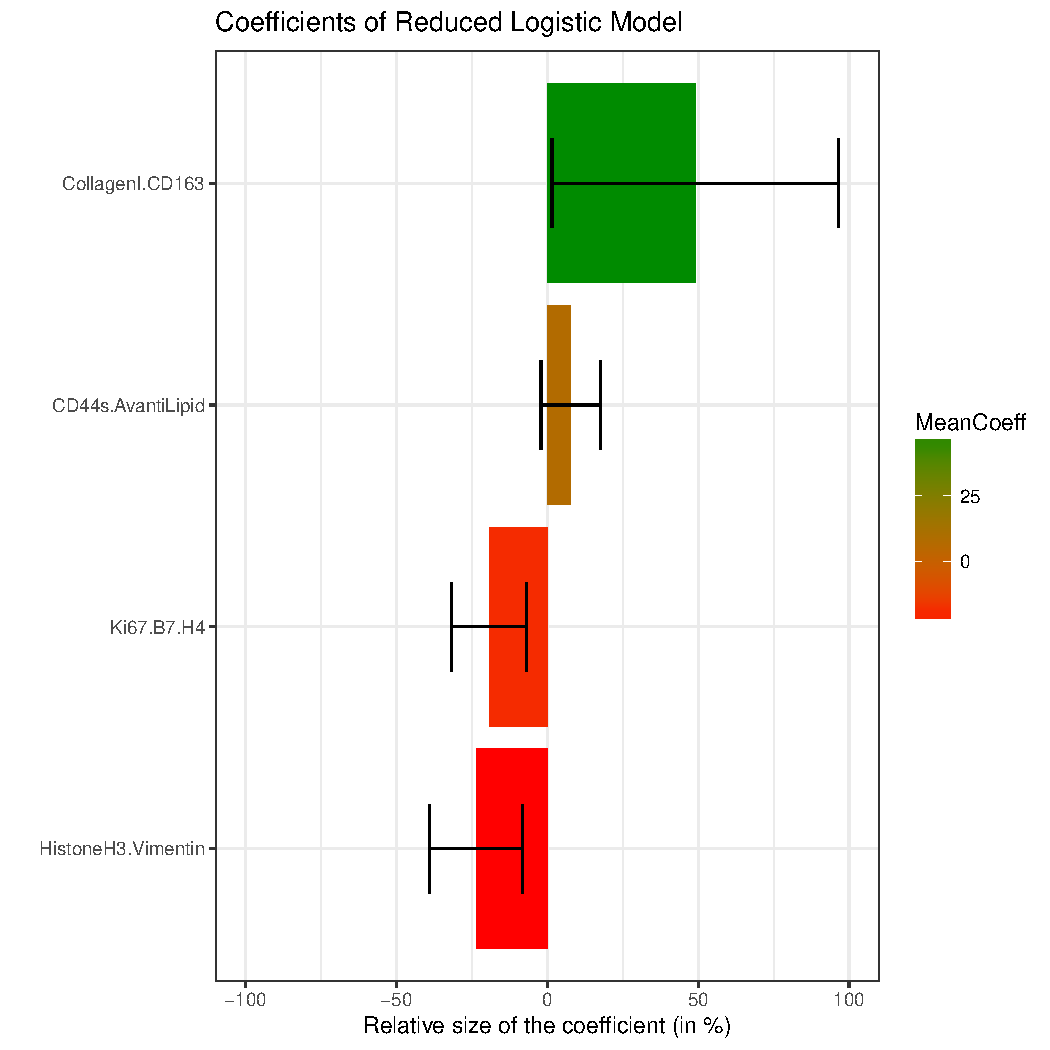
\includegraphics[width=\maxwidth]{figure/Fig_Model4Coef-1} \caption[Importance of the different stains according to the logistic model with maxVIF 100]{Importance of the different stains according to the logistic model with maxVIF 100. Asterisk indicates level of statistical support for non-zero contribution from this stain (T-test: *p$<$0.05,**p$<$0.01).}\label{fig:Fig_Model4Coef}
\end{figure}


\end{knitrout}

Alternatively there is a model with 13 coefficients:
\begin{knitrout}
\definecolor{shadecolor}{rgb}{0.969, 0.969, 0.969}\color{fgcolor}\begin{kframe}
\begin{alltt}
\hlstd{model13Coef} \hlkwb{=} \hlkwd{glm}\hlstd{(}\hlkwd{paste0}\hlstd{(best20[,}\hlnum{5}\hlstd{]),}\hlkwc{family}\hlstd{=}\hlkwd{binomial}\hlstd{(}\hlkwc{link}\hlstd{=}\hlstr{'logit'}\hlstd{),}
                           \hlkwc{data}\hlstd{=corrArrCurated_Reduced)}
\hlkwd{PlotCoefficients}\hlstd{(model13Coef,}\hlkwc{yLim}\hlstd{=}\hlkwd{c}\hlstd{(}\hlopt{-}\hlnum{100}\hlstd{,}\hlnum{100}\hlstd{),}\hlkwc{yPos}\hlstd{=}\hlnum{22}\hlstd{,}\hlkwc{errBarWidth}\hlstd{=}\hlnum{.4}\hlstd{)}
\end{alltt}
\end{kframe}\begin{figure}[h]
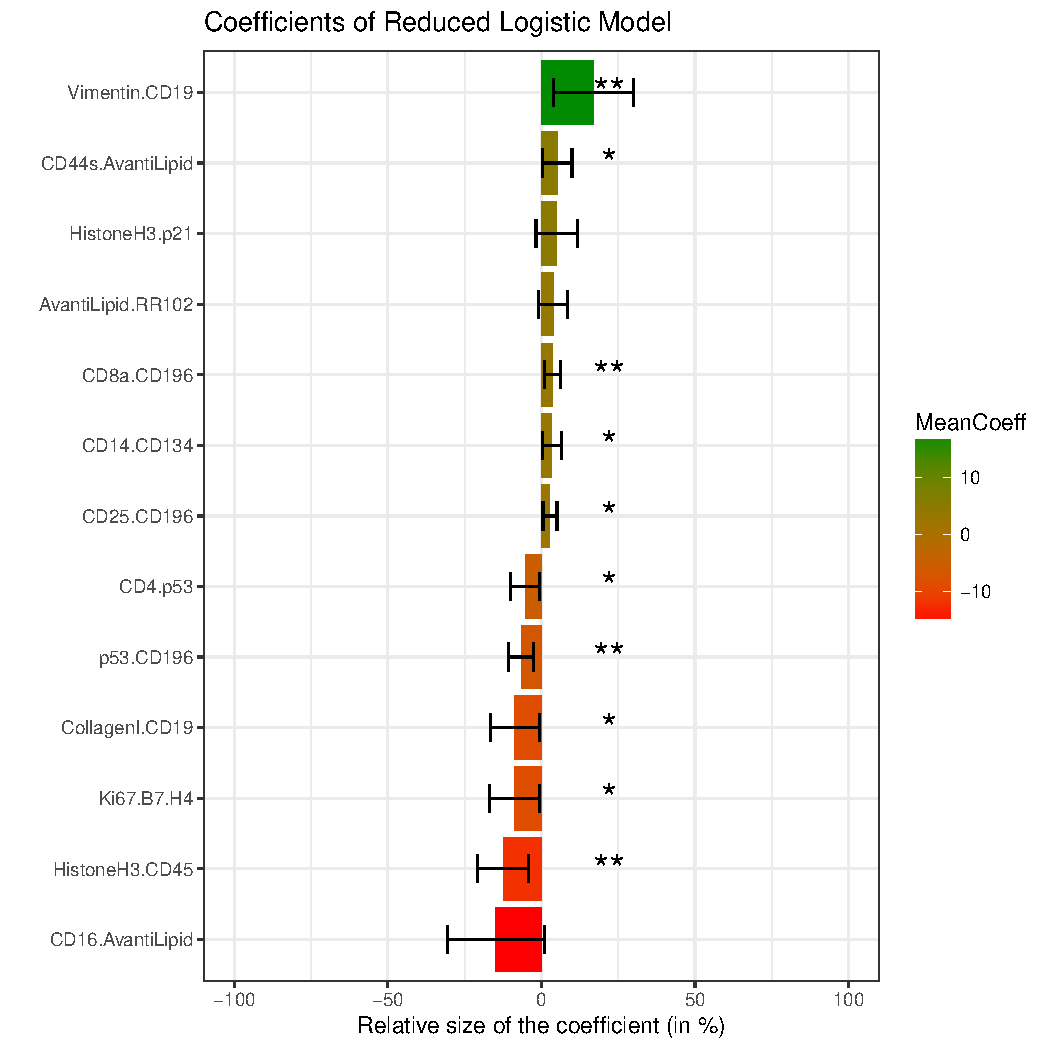
\includegraphics[width=\maxwidth]{figure/Fig_Model13Coef-1} \caption[Importance of the different stains according to the logistic model with maxVIF 100]{Importance of the different stains according to the logistic model with maxVIF 100. Asterisk indicates level of statistical support for non-zero contribution from this stain (T-test: *p$<$0.05,**p$<$0.01).}\label{fig:Fig_Model13Coef}
\end{figure}


\end{knitrout}

How do the two compare in cross-validation?
\begin{knitrout}
\definecolor{shadecolor}{rgb}{0.969, 0.969, 0.969}\color{fgcolor}\begin{kframe}
\begin{alltt}
\hlcom{# Cross-validation}
\hlstd{modelVec} \hlkwb{=} \hlkwd{c}\hlstd{(model4Coef}\hlopt{$}\hlstd{formula,model13Coef}\hlopt{$}\hlstd{formula)}
\hlstd{labelVec} \hlkwb{=} \hlkwd{c}\hlstd{(}\hlstr{"4 Coefficient Model"}\hlstd{,}
             \hlstr{"13 Coefficient Model"}\hlstd{)}
\hlkwd{PlotCrossValidation}\hlstd{(modelVec,corrArrCurated_Reduced,}\hlkwc{nIter}\hlstd{=}\hlnum{100}\hlstd{,}\hlkwc{nFolds}\hlstd{=}\hlnum{5}\hlstd{,}\hlkwc{labelVec}\hlstd{=labelVec)}
\end{alltt}
\end{kframe}\begin{figure}[h]
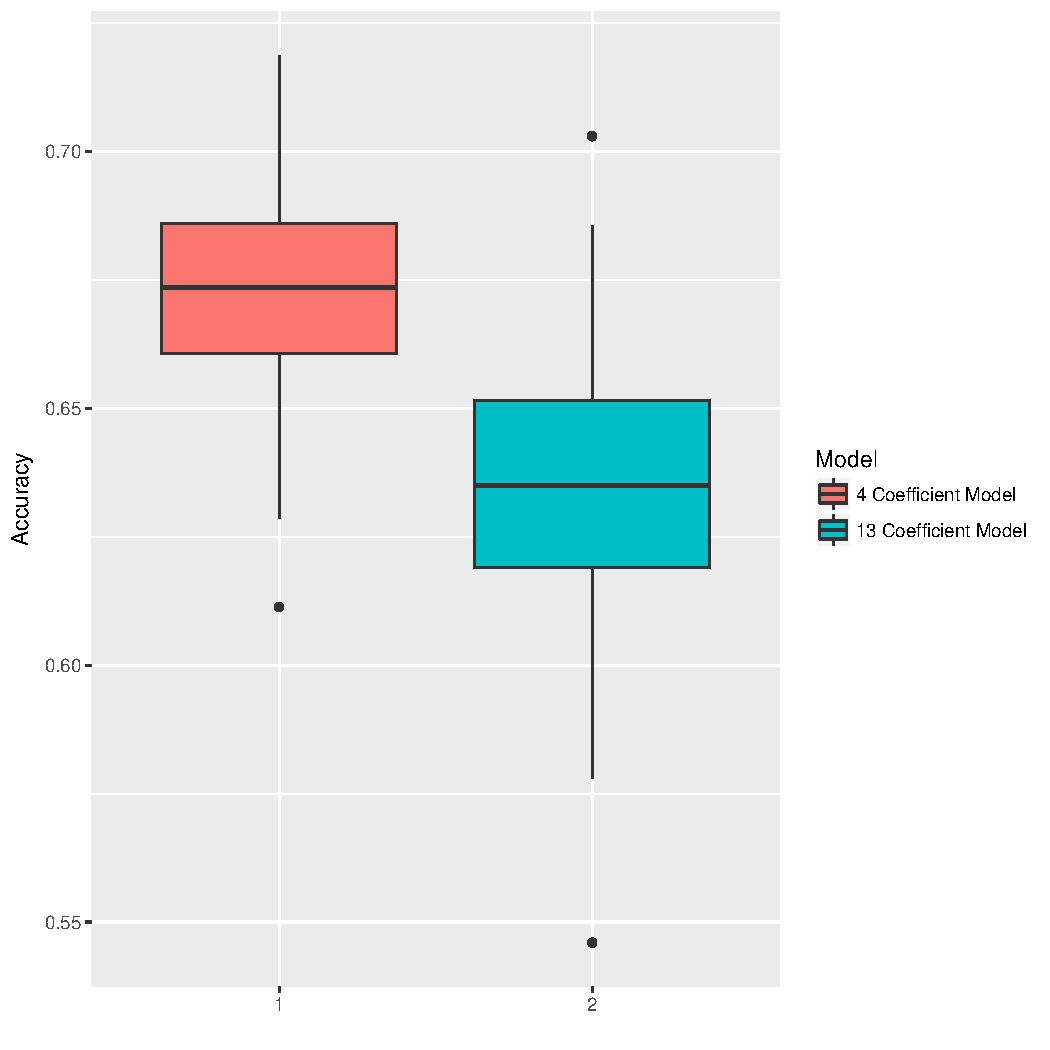
\includegraphics[width=\maxwidth]{figure/Fig_ModelComp1-1} \caption[Comparison of the model with 4 and the model with 13 coefficients in cross-validation (5-fold, 100 iterations)]{Comparison of the model with 4 and the model with 13 coefficients in cross-validation (5-fold, 100 iterations). Intriguingly the 4 Coefficient model does significantly better!}\label{fig:Fig_ModelComp1}
\end{figure}


\end{knitrout}

Interesting. The model with only 4 variables does much better than the one with 13. That's a bit strange. Maybe I should check the ROC curves? Anyhow, for now the results suggest that maybe macrophage infiltration and CD44s expression are positively related to response and B7H4 and Vimentin are negatively related. 

CD163 is a macrophage marker, so a strong collagen-cd163 correlation might indicate macrophage infiltration? 
CD44s is a membrane protein involved in cell-cell interactions. Thus, its correlation with AvantiLipid, which marks cell membranes is not too surprising. However, the fact that it is correlated with good outcome is something that the mean level model gives as well, and has been found in other studies as well. I see this as a little bit of a confirmation that we’re not just picking up noise. It shows that we’re picking up a correlation between two stains that we would expect to correlate and a result that is biologically valid as well.
B7H4 is a checkpoint inhibitor. Its interaction with Ki67 perhaps means that these cells are using this inhibitor for immune evasion?
Histones and vimentin perhaps hints at very aggressive tumour cells? Vimentin is part of the cytoskeleton and involved in actively moving cells.


In principle this could be interesting, however, it is not clear from this whether it's just because it likes the CD163 levels in general, or whether it is really about CD163 and Collagen being in the same place.

To if this is the case, let's first plot out the correlation for the patients to see if it really does separate them now and then colour in the images for those patients where the signal is strongest.

\begin{knitrout}
\definecolor{shadecolor}{rgb}{0.969, 0.969, 0.969}\color{fgcolor}\begin{kframe}
\begin{alltt}
\hlstd{only4CoefDataArr} \hlkwb{=} \hlstd{corrArrCurated_Reduced[,}\hlkwd{c}\hlstd{(}\hlstr{"CoreId"}\hlstd{,}\hlstr{"PtSnty"}\hlstd{,}\hlkwd{names}\hlstd{(model4Coef}\hlopt{$}\hlstd{coefficients)[}\hlopt{-}\hlnum{1}\hlstd{])]}
\hlstd{only4CoefDataArr} \hlkwb{=} \hlkwd{data.frame}\hlstd{(only4CoefDataArr,}\hlkwc{Prediction}\hlstd{=}\hlkwd{predict}\hlstd{(model4Coef,only4CoefDataArr,}\hlkwc{type}\hlstd{=}\hlstr{'response'}\hlstd{))}
\hlcom{# only4CoefDataArr[,2:5] = t(apply(only4CoefDataArr,1,function(row)\{row[-1]*model4Coef$coefficients[-1]\}))}
\hlstd{only4CoefDataArr} \hlkwb{=} \hlstd{only4CoefDataArr[}\hlkwd{with}\hlstd{(only4CoefDataArr,} \hlkwd{order}\hlstd{(PtSnty)), ]}
\hlstd{only4CoefDataArr_idxd} \hlkwb{=} \hlkwd{data.frame}\hlstd{(only4CoefDataArr,}\hlkwc{LinId}\hlstd{=}\hlkwd{seq}\hlstd{(}\hlkwd{nrow}\hlstd{(only4CoefDataArr)))}
\hlstd{only4CoefDataArr_reshaped} \hlkwb{=} \hlkwd{melt}\hlstd{(only4CoefDataArr_idxd[,}\hlopt{-}\hlnum{1}\hlstd{],}\hlkwc{id.vars}\hlstd{=}\hlkwd{c}\hlstd{(}\hlstr{"LinId"}\hlstd{))}
\hlkwd{ggplot}\hlstd{(only4CoefDataArr_reshaped,} \hlkwd{aes}\hlstd{(variable, LinId))} \hlopt{+}
  \hlkwd{geom_tile}\hlstd{(}\hlkwd{aes}\hlstd{(}\hlkwc{fill} \hlstd{= value),}\hlkwc{colour}\hlstd{=}\hlstr{"white"}\hlstd{)} \hlopt{+}
  \hlkwd{scale_fill_gradient}\hlstd{(}\hlkwc{low}\hlstd{=}\hlstr{"red"}\hlstd{,}\hlkwc{high}\hlstd{=}\hlstr{"blue"}\hlstd{)} \hlopt{+}
  \hlkwd{theme_bw}\hlstd{()} \hlopt{+}
  \hlkwd{labs}\hlstd{(}\hlkwc{x}\hlstd{=}\hlstr{""}\hlstd{,}\hlkwc{y}\hlstd{=}\hlstr{"Core"}\hlstd{)} \hlopt{+}
  \hlkwd{theme}\hlstd{(}\hlkwc{axis.text.x} \hlstd{=} \hlkwd{element_text}\hlstd{(}\hlkwc{angle}\hlstd{=}\hlnum{90}\hlstd{,} \hlkwc{hjust}\hlstd{=}\hlnum{1}\hlstd{))}
\end{alltt}
\end{kframe}\begin{figure}[h]
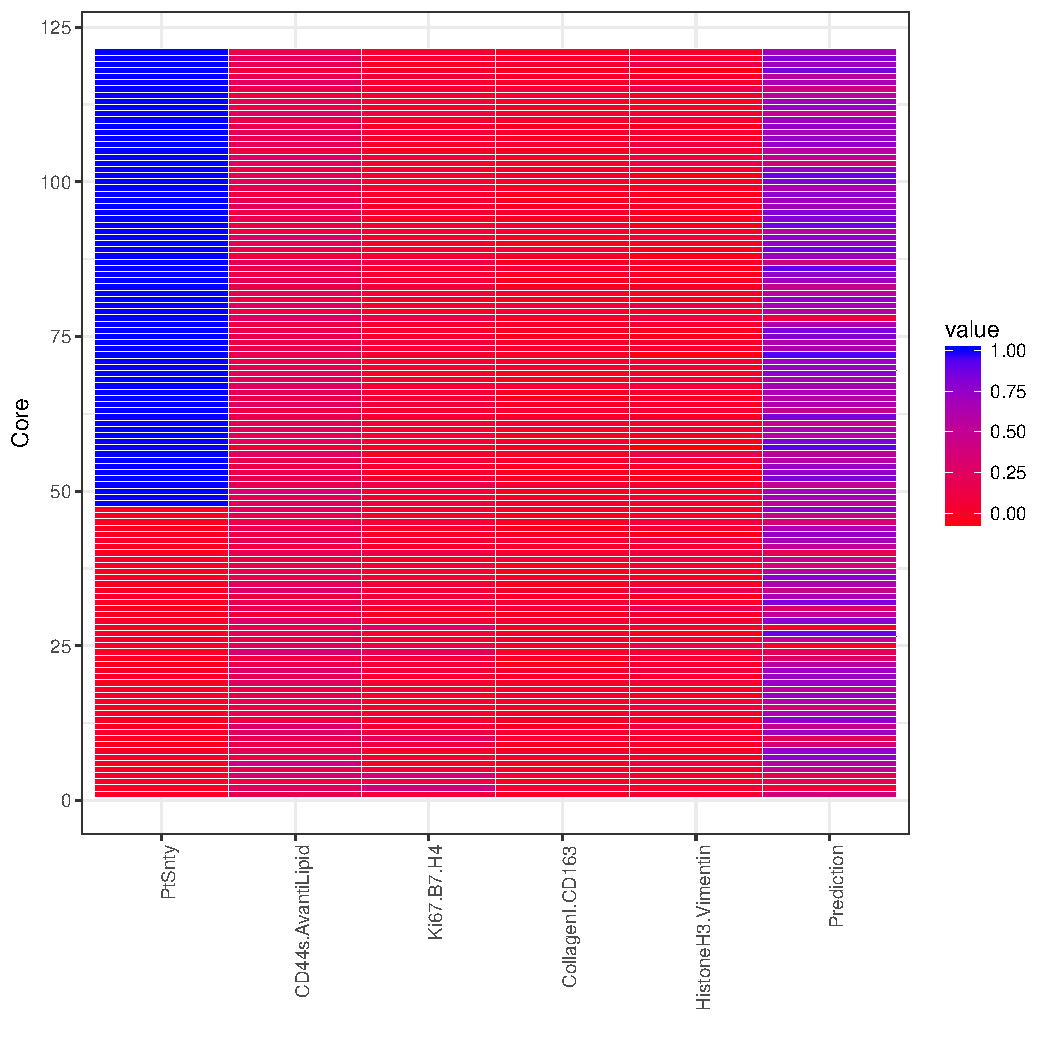
\includegraphics[width=\maxwidth]{figure/Fig_PatientTess-1} \end{figure}

\begin{kframe}\begin{alltt}
\hlcom{# predictions = ifelse(predictions > 0.5,1,0)}
\hlcom{# predictions==corrArrCurated_Reduced$PtSnty}
\hlcom{# }
\hlcom{# mean((predictions==0)[corrArrCurated_Reduced$PtSnty==0])}

\hlstd{only4CoefDataArr[}\hlkwd{which.min}\hlstd{(only4CoefDataArr}\hlopt{$}\hlstd{Prediction),]}
\end{alltt}
\begin{verbatim}
##    CoreId PtSnty CD44s.AvantiLipid Ki67.B7.H4 CollagenI.CD163
## 69    200      0         0.1864656  0.2755805    -0.002569898
##    HistoneH3.Vimentin Prediction
## 69          0.0420468 0.02315692
\end{verbatim}
\begin{alltt}
\hlstd{only4CoefDataArr[}\hlkwd{which.max}\hlstd{(only4CoefDataArr}\hlopt{$}\hlstd{Prediction),]}
\end{alltt}
\begin{verbatim}
##    CoreId PtSnty CD44s.AvantiLipid Ki67.B7.H4 CollagenI.CD163
## 38    161      1         0.1709083 0.03831591      0.02387417
##    HistoneH3.Vimentin Prediction
## 38         -0.0437627  0.9293528
\end{verbatim}
\begin{alltt}
\hlkwd{write.csv}\hlstd{(}\hlkwc{file}\hlstd{=}\hlstr{"correlationModelScores.csv"}\hlstd{,}\hlkwc{x}\hlstd{=only4CoefDataArr,}\hlkwc{row.names} \hlstd{=} \hlnum{FALSE}\hlstd{)}

\hlstd{only4CoefDataArr} \hlkwb{=} \hlstd{only4CoefDataArr[}\hlkwd{with}\hlstd{(only4CoefDataArr,} \hlkwd{order}\hlstd{(Prediction)), ]}
\end{alltt}
\end{kframe}
\end{knitrout}

What else might be helpful is to look at the images for patients with elevated correlations to see what they correspond to. Let's find a patient who has particularly high 


\end{document}
